\section{Key Exchange and Quantum Security}

\begin{frame}{Un po' di storia}

\framesubtitle{Come siamo arrivati qui}

\begin{itemize}%[<+->]
    \item 1994: Peter Shor pubblica un algoritmo (\cite{shor,shor2}) in grado di rompere RSA e altri schemi fattorizzando in primi in un modo impensabile per i computer classici
    \item 2005: Oded Regev pubblica una ricerca (\cite{regev}) sul problema del Learning With Errors
    \item 2016: Il NIST richiede nuovi standard in grado di resistere all'avvento del quantum computing
    \item 2017: Viene proposto CRYSTALS-Kyber (KEM) (\cite{ufficiale})
    \item 2018: Oded Regev vince il Premio Gödel per la sua ricerca
    \item 2021: CRYSTALS-Kyber è l'unico KEM reso standard (\cite{nistwinners})
    \item Esso è ora usato in varie applicazioni tra cui Signal, WhatsApp, un branch di OpenSSL e altri.
\end{itemize}

\end{frame}

\begin{frame}{Algoritmo di Shor}
\framesubtitle{Fattorizzazione quantistica}

\begin{itemize}%[<+->]
    \item La sicurezza di molti sistemi di crittografia asimmetrica o di scambio di chiavi si basa sulla difficoltà della fattorizzazione
    \item La difficoltà con l'algoritmo classico migliore che ci sia noto è al momento di \[
            O\left(e^{1.9(\log N)^{1/3}(\log\log N)^{2/3}}\right)
\]
    \item L'algoritmo di Shor (\cite{shor,shor2}), pubblicato nel 1994, è in grado di fattorizzare un numero in solo \[
    O\left((\log N)^2(\log\log N)\right)
\]
    \item Per ora non ancora applicabile su grandi numeri
    \item I computer quantistici continuano a migliorare (\cite{shorreal})
\end{itemize}
\end{frame}

\begin{frame}{Lattice-based Cryptography}
    \framesubtitle{Cosa è un lattice}

    \begin{colorblock}[black]{statalegrey}{Lattice}
Un lattice è, in geometria e nella teoria dei gruppi, un insieme infinito di punti in uno spazio vettoriale tale che la somma o sottrazione delle coordinate di due punti nel lattice produce le coordinate un terzo punto, sempre appartenente al lattice.
    \end{colorblock}

    Alcune costruzioni basate sui lattici (\cite{svp}) sembrano, al momento, resistenti ad attacchi (\cite{regev}) da parte di calcolatori non solo classici ma anche quantistici!

\end{frame}
\begin{frame}{Lattice-based Cryptography}
\framesubtitle{Learning With Errors}

    \begin{colorblock}[black]{statalegrey}{Learning with Errors}
        Il problema del Learning with Errors (LWE) (\cite{svp}) è un problema matematico basato sull'idea di rappresentare le informazioni come un insieme di equazioni aggiungendo del rumore, ossia degli errori.
    \end{colorblock}
    Esso è stato introdotto da Oded Regev nel suo lavoro del 2005 (\cite{regev}) ed è stato dimostrato avere la stessa complessità di molti problemi worst-case aventi a che fare con i lattici.
\end{frame}

\section{CRYSTALS-Kyber}

\begin{frame}{Public Key Encryption Scheme}
    Per avvicinarsi al KEM occorre costruire delle primitive da poter usare in seguito. Queste sono quelle tipiche della crittografia a chiave pubblica (\cite{kyber17}) ossia\begin{itemize}
    \item Key Generation
    \item Encryption
    \item Decryption
\end{itemize}
\end{frame}

\begin{frame}[fragile]{Key Generation}
    La generazione delle chiavi avviene nel seguente modo:

    \vspace{\baselineskip}

    \begin{minipage}{0.35\linewidth}
        %\begin{lstlisting}
        \begin{lstlisting}[title=Kyber.CPA.KeyGen():,mathescape=true]
$\rho,\sigma\leftarrow\{0,1\}^{256}$
$\boldsymbol{A}\sim R^{k\times k}_q:=\text{Sam}(\rho)$
$(\boldsymbol{s},\boldsymbol{e})\sim\beta^k_\eta\times\beta^k_\eta:=\text{Sam}(\sigma)$
$\boldsymbol{t}:=\text{Compress}_q(\boldsymbol{A}\boldsymbol{s}+\boldsymbol{e},d_t)$
$return (pk:=(\boldsymbol{t},\rho),sk:=\boldsymbol{s})$
        \end{lstlisting}
    \end{minipage}\hfill
    \begin{minipage}{0.6\linewidth}
        \begin{itemize}%[<+->]
            \item prendo due valori casuali $\rho,\sigma$ da $256$ bit
            \item genero una matrice $\boldsymbol{A}$ di dimensioni $k\times k$ con coefficienti modulo $q$ a partire da $\rho$
            \item ottengo i valori di chiave privata $s$ ed errore $e$ come array di dimensione $k$ con coefficienti piccoli (modulo $\eta$) a partire da $\sigma$
            \item ottengo $t$ come compressione di $\boldsymbol{A}\boldsymbol{s}+\boldsymbol{e}$
            \item restituisco la coppia chiave pubblica, chiave privata
        \end{itemize}
    \end{minipage}

\end{frame}

\begin{frame}[fragile]{Encryption}
    \framesubtitle{Parte A}
    \begin{minipage}{0.45\linewidth}
        %\begin{lstlisting}
        \begin{lstlisting}[title={Kyber.CPA.Enc(pk,m):},mathescape=true]
$r\leftarrow\{0,1\}^{256}$
$\boldsymbol{t}:=\text{Decompress}_q(\boldsymbol{t},d_t)$
$\boldsymbol{A}\sim R^{k\times k}_q:=\text{Sam}(\rho)$
$(\boldsymbol{r},\boldsymbol{e_1},e_2)\sim\beta^k_\eta\times\beta^k_\eta\times\beta_\eta:=\text{Sam}(r)$
...
        \end{lstlisting}
    \end{minipage}\hfill
    \begin{minipage}{0.5\linewidth}
        \begin{itemize}%[<+->]
            \item creo un valore casuale di inizializzazione $r$
            \item ottengo $\boldsymbol{t}$ dal parametro compresso ottenuto in input ($pk=(\boldsymbol{t},\rho)$)
            \item mi ricostruisco la matrice $\boldsymbol{A}$ usando una Extendable Output Function a partire sempre da $\rho$ (si ricorda che le funzioni Sam sono deterministiche)
            \item ottengo $\boldsymbol{r},\boldsymbol{e_2},e_2$ come due array di polinomi e un polinomio con coefficienti \textit{piccoli}

        \end{itemize}
    \end{minipage}
\end{frame}

\begin{frame}[fragile]{Encryption}
    \framesubtitle{Parte B}
    \begin{minipage}{0.45\linewidth}
        %\begin{lstlisting}
        \begin{lstlisting}[title={Kyber.CPA.Enc(pk,m):},mathescape=true,firstnumber=4]
...
$\boldsymbol{u}:=\text{Compress}_q(\boldsymbol{A}^T\boldsymbol{r}+\boldsymbol{e_1},d_u)$
$v:=\text{Compress}_q(\boldsymbol{t}^T\boldsymbol{r}+e_2+\left\lceil\frac{q}{2}\right\rfloor\cdot m,d_v)$
$\text{return }c:=(\boldsymbol{u},v)$
        \end{lstlisting}
    \end{minipage}\hfill
    \begin{minipage}{0.5\linewidth}
        \begin{itemize}%[<+->]
            \item calcolo $\boldsymbol{u}$ usando gli errori vettoriali generati precedentemente
            \item calcolo $v$ comprimendo il risultato della somma di rumore da due fonti ($\boldsymbol{t}^T\boldsymbol{r}$,$e_2$) e il messaggio appositamente amplificato in modo che abbia coefficienti grandi
            \item restituisco il ciphertext, ossia la coppia $(\boldsymbol{u},v)$
        \end{itemize}
    \end{minipage}
\end{frame}

\begin{frame}[fragile]{Decryption}

    \vspace{\baselineskip}

    \begin{minipage}{0.35\linewidth}
        %\begin{lstlisting}
        \begin{lstlisting}[title={Kyber.CPA.Dec(sk,c):},mathescape=true]
$\boldsymbol{u}:=\text{Decompress}_q(\boldsymbol{u},d_u)$
$v:=\text{Decompress}_q(v,d_v)$
$\text{return Compress}_q(v-\boldsymbol{s}^T\boldsymbol{u},1)$
        \end{lstlisting}
    \end{minipage}\hfill
    \begin{minipage}{0.6\linewidth}
        \begin{itemize}%[<+->]
            \item ottengo $\boldsymbol{u}$ e $v$ decomprimendo il ciphertext
            \item ricavo il plaintext come $v-\boldsymbol{s}^T\boldsymbol{u}$ e approssimando: se il valore del coefficiente è più vicino a $0$ o $q$ che a $\left\lceil\frac{q}{2}\right\rfloor$ allora avrò uno $0$, altrimenti un $1$
        \end{itemize}
    \end{minipage}

\end{frame}

\begin{frame}{Messaggi e polinomi}
    Noi siamo abituati a trasmettere i messaggi nella forma di numeri, tuttavia qui lavoriamo con i polinomi. Come è possibile questo?

    \begin{block}{I numeri sono polinomi}
        Ci basta effettuare una semplice conversione prendendo il messaggio in binario e associando ad ogni bit un esponente, ad esempio $11_{10}=1011_2=x^3+x+1$ (\cite{kyber17,babykyber}).
    \end{block}

    \begin{colorblock}{statalegreen}{Amplificazione del polinomio}
        Per evitare che i rumori introdotti come parte fondamentale della crittografia vadano a sovrascrivere il nostro messaggio rendendolo inintellegibile amplifichiamo il nostro messaggio di una quantità pari alla metà di $q$, così lo riusciamo a distinguere (\cite{kyber17,babykyber}). Questo risulta evidente dallo pseudocodice dell'encryption.
    \end{colorblock}
\end{frame}

    \begin{frame}{Correttezza di Kyber.CPA}

    \begin{colorblock}{stataleyellow}{Correttezza}
        Kyber.CPA è $(1-\delta)-$corretto con un $\delta<2^{-128}$ (\cite{kyber17}). Questo significa che una piccola quantità di decryption potrebbero non portare al valore realmente desiderato. Questa quantità è però trascurabile.
    \end{colorblock}

    \end{frame}

\begin{frame}{Costruire un KEM}
    \framesubtitle{Premessa}
    Per costruire un KEM dovremo usare le primitive di Key Exchange costruite prima per ottenere due funzionalità:\begin{itemize}
    \item Encaps: questa funzione ci fornirà la chiave da proporre e un ciphertext avendo a disposizione una chiave pubblica
    \item Decaps: questa funzione prende in input una chiave privata e un ciphertext e ottiene la chiave concordata
    \end{itemize}
    Esso ovviamente necessita anche di KeyGen, che tuttavia rimane identico a prima (\cite{kyber17})
\end{frame}

    \begin{frame}[fragile]{Encaps}
\begin{minipage}{0.45\linewidth}
        %\begin{lstlisting}
    \begin{lstlisting}[title=Kyber.Encaps(pk):,mathescape=true]
$m\leftarrow\{0,1\}^{256}$
$(\hat{K},r):=G(H(pk),m)$
$(\boldsymbol{u},v):=\text{Kyber.CPA.Enc}((\boldsymbol{t},\rho),m;r)$
$c:=(\boldsymbol{u},v)$
$K:=H(\hat{K},H(c))$
return $(c,K)$
        \end{lstlisting}
    \end{minipage}\hfill
    \begin{minipage}{0.5\linewidth}
        \begin{itemize}%[<+->]
            \item genero un valore casuale $m$
            \item ottengo il seme dei numeri casuali e parte della chiave dagli hash di $m$
            \item cifro il valore $m$ usando $r$ come seme
            \item uso sia il ciphertext che il plaintext per ottenere la chiave
            \item trasmetto il ciphertext            
        \end{itemize}
    \end{minipage}
    \end{frame}

        \begin{frame}[fragile]{Decaps}
            \framesubtitle{Parte A}
\begin{minipage}{0.45\linewidth}
        %\begin{lstlisting}
    \begin{lstlisting}[title=Kyber.Decaps(sk\,z\,c):,mathescape=true]
$m':=\text{Kyber.CPA.Dec}(s,(\boldsymbol{u},v))$
$(\hat{K}',r'):=G(H(pk),m')$
$(\boldsymbol{u}',v'):=\text{Kyber.CPA.Enc}((\boldsymbol{t},\rho),m';r')$
...
        \end{lstlisting}
    \end{minipage}\hfill
    \begin{minipage}{0.5\linewidth}
        \begin{itemize}%[<+->]
            \item decifro il messaggio che mi è arrivato
            \item ottengo il seed e la $\hat{K}'$
            \item provo a cifrare nuovamente con gli stessi parametri (ho eliminato il non determinismo della cifratura)
        \end{itemize}
    \end{minipage}
        \end{frame}

\begin{frame}[fragile]{Decaps}
            \framesubtitle{Parte B}
\begin{minipage}{0.45\linewidth}
        %\begin{lstlisting}
    \begin{lstlisting}[title=Kyber.Decaps(sk\,z\,c):,mathescape=true,firstnumber=3]
...
if $(\boldsymbol{u}',v') == (\boldsymbol{u},v)$ then
    return $K:=H(\hat{K}',H(c))$
else
    return $K:=H(z,H(c))$
end if
    \end{lstlisting}
    \end{minipage}\hfill
    \begin{minipage}{0.5\linewidth}
        \begin{itemize}%[<+->]
            \item se il ciphertext coincide allora restituisco la chiave
            \item altrimenti restituisco una chiave sbagliata generata a partire da $z$
        \end{itemize}
    \end{minipage}
        \end{frame}



\begin{frame}{Funzioni di Hashing}
    Per eseguire alcune operazioni nell'incapsulamento e decapsulamento si fa uso di funzioni di hashing. Seguendo l'articolo \cite{kyber17} noi useremo due varianti Keccak, ossia \texttt{sha3-256} come $H$ e \texttt{sha3-512} come $G$, il cui output sarà trasformato in polinomi seguendo le solite regole.
\end{frame}

\section{Baby-Kyber KEM}

\begin{frame}{Una versione ridotta}
    \framesubtitle{Un esempio concreto e una implementazione}
    \begin{colorblock}{stataleyellow}{Avviso}
        Per vedere un esempio ridotto fare riferimento a \cite{babykyber}. L'uso di parametri così bassi potrebbe aumentare il tasso di errori. Inoltre, questo sistema non fa uso di compressione, a differenza del vero CRYSTALS-Kyber \cite{kyber17,ufficiale}.
    \end{colorblock}

    Qui non sarà riportata questa versione quanto una rappresentazione del protocollo specifico realizzato come componente chiave del sistema di chat LightKnife.

\end{frame}

    \section{Man in the Middle and Key Exchange Scenarios}

\begin{frame}{Kyber.KE protocol}
    \framesubtitle{Logical view}

\begin{center}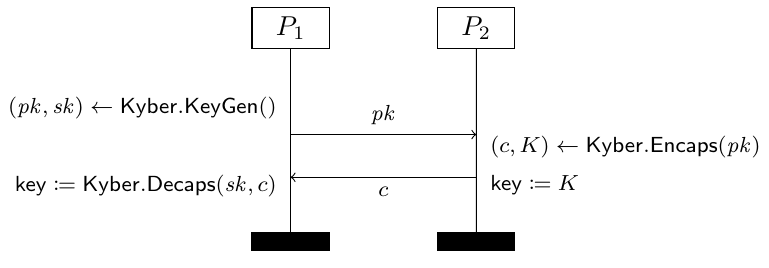
\includegraphics[scale=0.6]{./assets/logical_view.png}\end{center}

\end{frame}

    \begin{frame}{Kyber.KE protocol}
    \framesubtitle{Network view}

    \begin{center}
    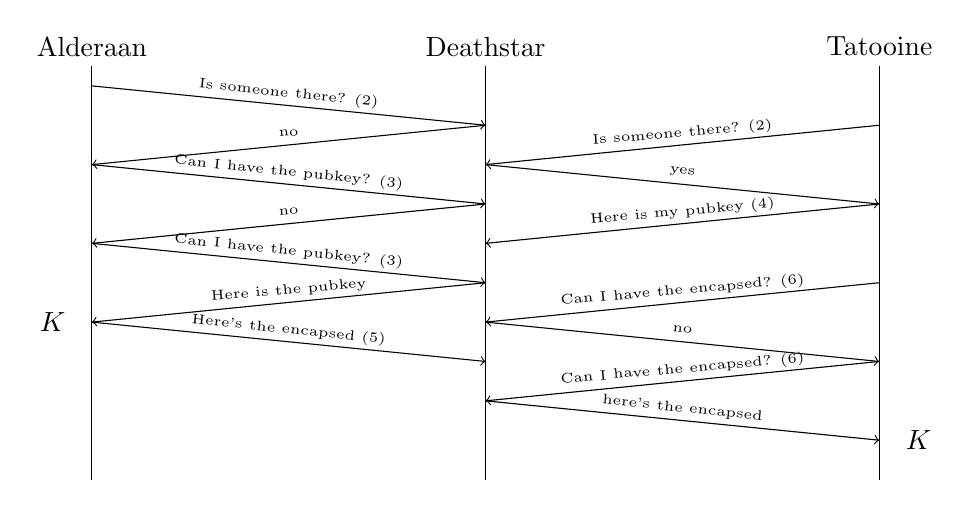
\begin{tikzpicture}
        \node[] at (0,0) (alderaan) {Alderaan};
        \node[] at (5,0) (deathstar) {Deathstar};
        \node[] at (10,0) (tatooine) {Tatooine};
        \node[] at (0,-5.5) (endlines) {};
        \draw[-] (alderaan.south) -- (alderaan.south|-endlines);
        \draw[-] (deathstar.south) -- (deathstar.south|-endlines);
        \draw[-] (tatooine.south) -- (tatooine.south|-endlines);
        
        \draw[->] (0,-0.5) -- (5,-1);
        \node[] at (2.5,-0.6) (text1) {\rotatebox{-6}{\tiny Is someone there? (2)}};
        \draw[->] (5,-1) -- (0,-1.5);
        \node[] at (2.5,-1.1) (text1) {\rotatebox{5}{\tiny no}};
        \draw[->] (0,-1.5) -- (5,-2);
        \node[] at (2.5,-1.6) (text1) {\rotatebox{-6}{\tiny Can I have the pubkey? (3)}};
        \draw[->] (5,-2) -- (0,-2.5);
        \node[] at (2.5,-2.1) (text1) {\rotatebox{5}{\tiny no}};
        \draw[->] (0,-2.5) -- (5,-3);
        \node[] at (2.5,-2.6) (text1) {\rotatebox{-6}{\tiny Can I have the pubkey? (3)}};
        \draw[->] (5,-3) -- (0,-3.5);
        \node[] at (2.5,-3.1) (text1) {\rotatebox{5}{\tiny Here is the pubkey}};
        \draw[->] (0,-3.5) -- (5,-4);
        \node[] at (2.5,-3.6) (text1) {\rotatebox{-6}{\tiny Here's the encapsed (5)}};
        \node[] at (-0.5,-3.5) (k) {$K$};

        \draw[->] (10,-1) -- (5,-1.5);
        \node[] at (7.5,-1.1) (text1) {\rotatebox{5}{\tiny Is someone there? (2)}};
        \draw[->] (5,-1.5) -- (10,-2);
        \node[] at (7.5,-1.6) (text1) {\rotatebox{-6}{\tiny yes}};
        \draw[->] (10,-2) -- (5,-2.5);
        \node[] at (7.5,-2.1) (text1) {\rotatebox{5}{\tiny Here is my pubkey (4)}};
        \draw[->] (10,-3) -- (5,-3.5);
        \node[] at (7.5,-3.1) (text1) {\rotatebox{5}{\tiny Can I have the encapsed? (6)}};
        \draw[->] (5,-3.5) -- (10,-4);
        \node[] at (7.5,-3.6) (text1) {\rotatebox{-6}{\tiny no}};
        \draw[->] (10,-4) -- (5,-4.5);
        \node[] at (7.5,-4.1) (text1) {\rotatebox{5}{\tiny Can I have the encapsed? (6)}};
        \draw[->] (5,-4.5) -- (10,-5);
        \node[] at (7.5,-4.6) (text1) {\rotatebox{-6}{\tiny here's the encapsed}};
        \node[] at (10.5,-5) (k) {$K$};

    \end{tikzpicture}
    \end{center}

        \cite{kyber17}
\end{frame}

    \begin{frame}{Man in the Middle against Kyber.KE}
    \begin{center}
    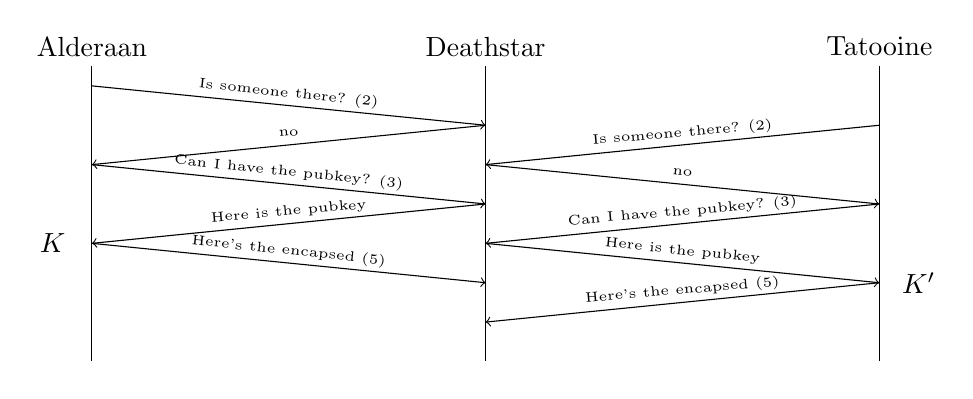
\begin{tikzpicture}
        \node[] at (0,0) (alderaan) {Alderaan};
        \node[] at (5,0) (deathstar) {Deathstar};
        \node[] at (10,0) (tatooine) {Tatooine};
        \node[] at (0,-4) (endlines) {};
        \draw[-] (alderaan.south) -- (alderaan.south|-endlines);
        \draw[-] (deathstar.south) -- (deathstar.south|-endlines);
        \draw[-] (tatooine.south) -- (tatooine.south|-endlines);

        \draw[->] (0,-0.5) -- (5,-1);
        \node[] at (2.5,-0.6) (text1) {\rotatebox{-6}{\tiny Is someone there? (2)}};
        \draw[->] (5,-1) -- (0,-1.5);
        \node[] at (2.5,-1.1) (text1) {\rotatebox{5}{\tiny no}};
        \draw[->] (0,-1.5) -- (5,-2);
        \node[] at (2.5,-1.6) (text1) {\rotatebox{-6}{\tiny Can I have the pubkey? (3)}};
        \draw[->] (5,-2) -- (0,-2.5);
        \node[] at (2.5,-2.1) (text1) {\rotatebox{5}{\tiny Here is the pubkey}};
        \draw[->] (0,-2.5) -- (5,-3);
        \node[] at (2.5,-2.6) (text1) {\rotatebox{-6}{\tiny Here's the encapsed (5)}};
        \node[] at (-0.5,-2.5) (k) {$K$};

        \draw[->] (10,-1) -- (5,-1.5);
        \node[] at (7.5,-1.1) (text1) {\rotatebox{5}{\tiny Is someone there? (2)}};
        \draw[->] (5,-1.5) -- (10,-2);
        \node[] at (7.5,-1.6) (text1) {\rotatebox{-6}{\tiny no}};
        \draw[->] (10,-2) -- (5,-2.5);
        \node[] at (7.5,-2.1) (text1) {\rotatebox{5}{\tiny Can I have the pubkey? (3)}};
        \draw[->] (5,-2.5) -- (10,-3);
        \node[] at (7.5,-2.6) (text1) {\rotatebox{-6}{\tiny Here is the pubkey}};
        \draw[->] (10,-3) -- (5,-3.5);
        \node[] at (7.5,-3.1) (text1) {\rotatebox{5}{\tiny Here's the encapsed (5)}};
        \node[] at (10.5,-3) (k) {$K'$};

        
    \end{tikzpicture}
    \end{center}

    \end{frame}

    \begin{frame}{Kyber.UAKE and Kyber.AKE}
        \begin{minipage}{0.45\linewidth}
            \begin{center}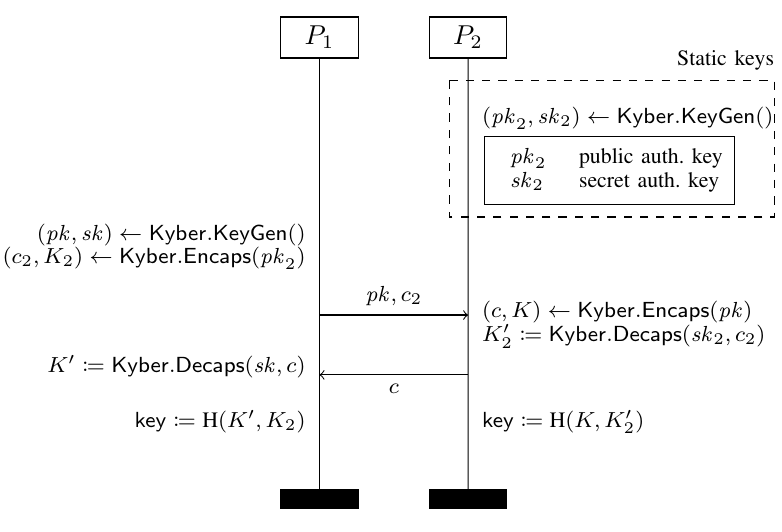
\includegraphics[scale=0.3]{./assets/uake.png}\end{center}

            One-side Authenticated Key Exchange
        \end{minipage}\hfill\begin{minipage}{0.45\linewidth}
            \begin{center}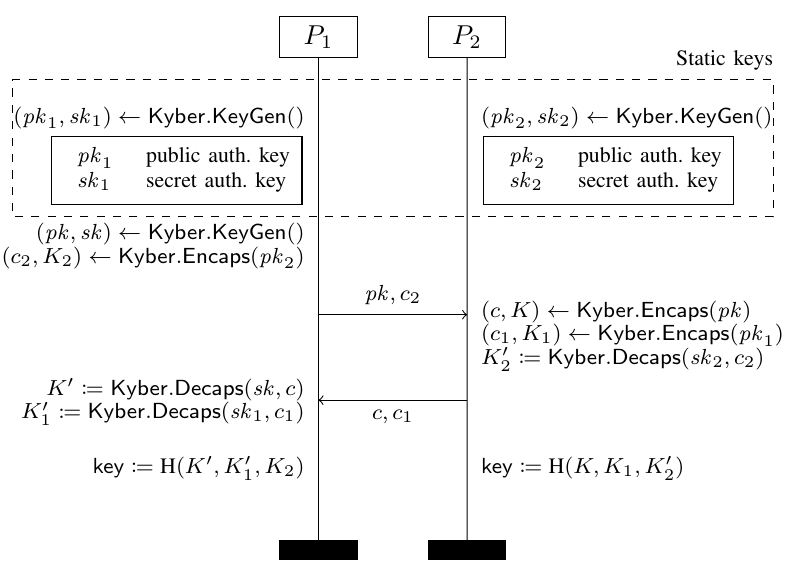
\includegraphics[scale=0.3]{./assets/ake.png}\end{center}

        Authenticated Key Exchange
        \end{minipage}
        
        \cite{kyber17}
    \end{frame}

